\documentclass[11pt,a4paper]{article}

\newcommand{\hc} {HC}

\newcommand{\hp} {HP}

\usepackage{tikz}

%%% front matter

  \title{Coursework 4: Graph Algorithms and Complexity Theory}
  \author{Oskar Mampe}
  \date{Tutorial Session: Thursday 1pm}

\begin{document}

\maketitle
\thispagestyle{empty}

\textbf{Explanation: } A \textit{hamiltonian path} in an undirected graph is a path that contains all vertices of the graph (without repetition).  Similarly, a \textit{hamiltonian cycle} is a cycle that contains all vertices of the graph.  A graph with hamiltonian path is \textit{traceable}, and a graph with hamiltonian cycle is \textit{hamiltonian}.

\begin{enumerate}
    \item Specify decision problems \hp{} and \hc{}  dealing with hamiltonian paths and hamiltonian cycles in undirected graphs.
    
    \hp{}:\\ Input: An undirected graph $G = (V, E)$.\\ Question: Does $G$ contain a Hamiltonian Path?\\


    \hc{}:\\ Input: An undirected graph $G = (V, E)$.\\ Question: Does $G$ contain a Hamiltonian Circuit?\\

    \item Show \hp{} $\leq^p_m$ \hc{} by completing the following tasks: 
        \begin{enumerate}
            \item Construct a polynomial transformation $f$ from \hp{} to \hc{}.\\
            Let $G = (V, E)$ be an input for a hamiltonian path. Let $f(G) = G'  = (V', E')$,
             where $V' = V \cup \{v\}$ $v \notin V$ and $E' = E \; \cup  \; \{ \{ v, w\} | w \in V\}$.
             This is in polynomial time as adding a vertex takes constant time and adding edges $\{v, w \}$
              for all $w \in V$ takes $|V|$ amount of time. In total this operation takes $|V| + c$ amount of time, which is in polynomial time. 
              \begin{center}
                \begin{tikzpicture}[scale=0.5]
                    \node (A) at (2.5,-3) {$v_1$};
                    \node (C) at (0,3) {$v_2$};
                    \node (D) at (2.5,4) {$v_3$};
                    \node (B) at (0,0) {$v_4$};
                    \node (E) at (5,3) {$v_5$};

                    \path (A) edge node {} (B);
                    \path (B) edge node {} (C);
                    \path (C) edge node {} (D);
                    \path (D) edge node {} (E);
                \end{tikzpicture}
                \raisebox{20mm}[0pt][0pt]{%
                \makebox[1em][c]{$\Rightarrow$}}
                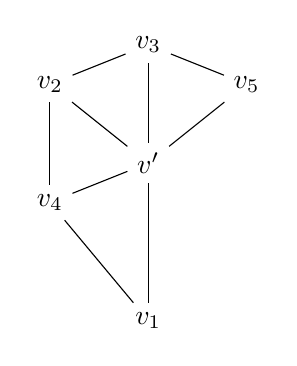
\begin{tikzpicture}[scale=0.5]
                    \node (A) at (2.5,-3) {$v_1$};
                    \node (C) at (0,3) {$v_2$};
                    \node (D) at (2.5,4) {$v_3$};
                    \node (B) at (0,0) {$v_4$};
                    \node (E) at (5,3) {$v_5$};
                    \node (F) at (2.5,1) {$v'$};

                    \path (A) edge node {} (B);
                    \path (B) edge node {} (C);
                    \path (C) edge node {} (D);
                    \path (D) edge node {} (E);

                    \path (F) edge node {} (A);
                    \path (F) edge node {} (B);
                    \path (F) edge node {} (C);
                    \path (F) edge node {} (D);
                    \path (F) edge node {} (E);

                \end{tikzpicture}
            \end{center}
            \item Show for all graphs $G$ that $G \in Y_{\hp{}} \Rightarrow f(G) \in Y_{\hc{}}$.\\
            \textbf{Proof:} Let $G \in \hp{}$.
            Given a path $p = (v_1, \ldots, v_n)$ of $G$ connect the vertex $v_n$ to $v_1$ through $v'$,
              making a path $p' = (v_1, \ldots, v_n, v', v_1)$, which is a cycle.
               The vertices $v_n$ and $v_1$ will always be able to traverse to $v'$
                as $v'$ is connected to all vertices. $f(G) \in Y_{\hc{}}$ as it is a hamiltonian path that starts and ends at the vertex $v_1$.\\
            
            \item Show for all graphs $G$ that $f(G) \in Y_{\hc{}} \Rightarrow G \in Y_{\hp{}}$.\\
            \textbf{Proof:} Let $f(G) \in \hc{}$. Given a path $p' = (v_1, \ldots, v_{n-1}, v_n, v_1)$ removing $v_n, v_1$ gives $p'' = (v_1, \ldots, v_{n-1})$.
            The result has to be a path as $v_n$ will always be the bridge between the last node of a hamiltonian path and the first. If the endpoints of the path are not known, then a vertex with degree $|V|$ can be assumed as $v'$.
            
            
        \end{enumerate}
    \item Show \hc{} $\leq^p_m$ \hp{} by completing the following tasks: 
    \begin{enumerate}
        \item Construct a polynomial transformation $g$ from \hc{} to \hp{}.\\
        Let $G = (V, E)$ be an input for a Hamiltonian Cycle. Let $g(G) = G'  = (V', E')$,
             where $v \in V$ is a vertex in $G$, $V' = V \cup \{v', s, t\}$  where $v', s, t \notin V$ and $E' = E \cup \{ \{v',w\} | \{v, w\} \in E \} \cup \{ \{ t, v' \}, \{s, v\}, \{v, v'\} \}$.
             This is in polynomial time as adding 3 vertices takes constant time and adding edges $\{ \{v',w\} | \{v, w\} \in E \} \cup \{ \{ t, v' \}, \{s, v\}, \{v, v'\} \}$
            takes $|V| + c$ amount of time, which is in polynomial time. \\
            \begin{center}
            \raisebox{5mm}[0pt][0pt]{
         \begin{tikzpicture}[scale=0.5]
            \node (A) at (2,0) {$v_1$};
            \node (B) at (-1,3) {$v_2$};
            \node (C) at (2.5,4.5) {$v_3$};
            \node (D) at (5,3) {$v_4$};

            \path (A) edge node {} (B);
            \path (B) edge node {} (C);
            \path (C) edge node {} (D);
            \path (D) edge node {} (A);
        \end{tikzpicture}
        }
        \raisebox{20mm}[0pt][0pt]{%
                \makebox[1em][c]{$\Rightarrow$}}
        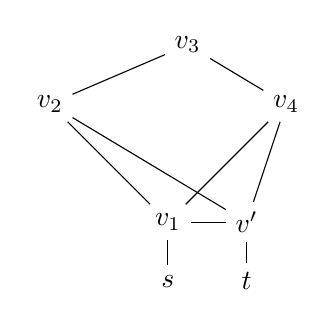
\begin{tikzpicture}[scale=0.5]
            \node (A) at (2,0) {$v_1$};
            \node (B) at (-1,3) {$v_2$};
            \node (C) at (2.5,4.5) {$v_3$};
            \node (D) at (5,3) {$v_4$};
            \node (E) at (4,0) {$v'$};
            \node (S) at (2,-1.5) {$s$}; 
            \node (T) at (4,-1.5) {$t$}; 

            \path (A) edge node {} (B);
            \path (B) edge node {} (C);
            \path (C) edge node {} (D);
            \path (A) edge node {} (D);
            \path (E) edge node {} (A); 
            \path (E) edge node {} (B); 
            \path (E) edge node {} (D);
            \path (A) edge node {} (S);
            \path (E) edge node {} (T);
            
        \end{tikzpicture}\\
    \end{center}
        \item Show for all graphs $G$ that $G \in Y_{\hc{}} \Rightarrow g(G) \in Y_{\hp{}}$.\\
        \textbf{Proof:} Given a path where $p = (v_1, u, \dots, y, v_1)$ which traverses all the vertices and end up at the same vertex $v_1$. 
         However, if you create a copy $v'$ of $v$ and then connect $s$ to $v$ and $t$ to $v'$, as $s, t$ being the endpoints this must translate to a hamiltonian path,
         making the path $p' = (s,v,u,\ldots , y, v', t)$. Considering s and t are only connected to the one vertex, the path must begin and end at these vertices.\\
        \item Show for all graphs $G$ that $g(G) \in Y_{\hp{}} \Rightarrow G \in Y_{\hc{}}$.\\
        \textbf{Proof:} Given a path in $g(G)$, it is guaranteed that $s, t$ are the endpoints. Therefore, ignoring the first and last edge of the path will give you the path $c' = (v,u,\ldots , y', v')$, which is a path from the first vertex $v$  to the copy of the first vertex $v'$. Merging $v$ and $v'$ will give back the graph $G \in Y_{\hc}$ with the original cycle. 
    \end{enumerate}
\end{enumerate}

\end{document}
    